\chapter{Additional Design and Architectural Diagrams}
\label{app:diagrams}

This appendix provides supplementary models of the generative workflow and of the combat-feedback event flow.

\section{Two-Stage Decoupled Dungeon Generation Pipeline}
Figure~\ref{fig:two_stage_detail} illustrates the strict separation of concerns between Stage 1 topological floor synthesis and Stage 2 PPO combat encounter population.

\begin{figure}[!htbp]
\centering
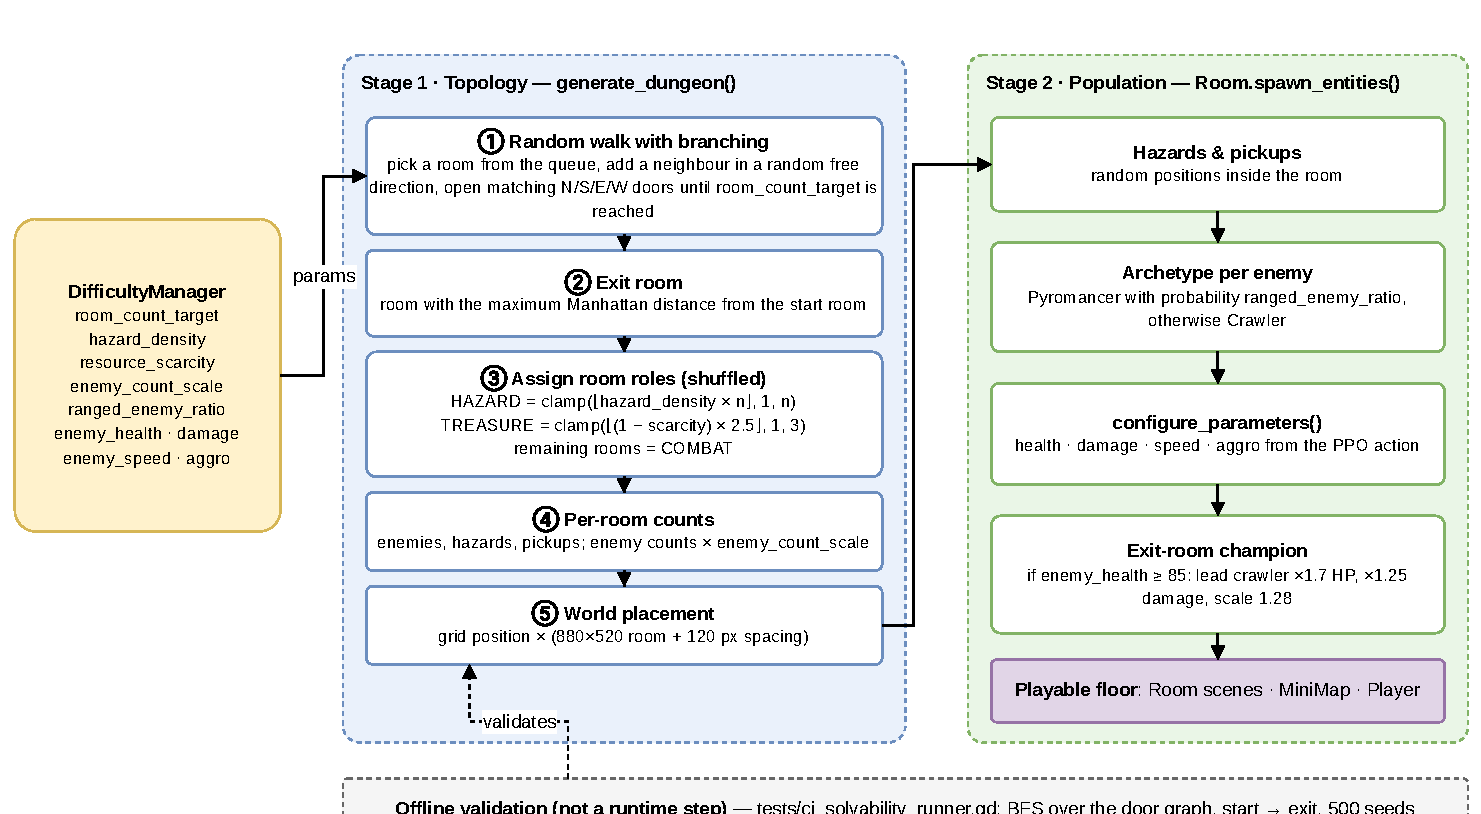
\includegraphics[width=0.95\textwidth]{ThesisFigs/fig_e_1_two_stage_procedural_pipeline}
\caption{Two-Stage Decoupled Procedural Generation Pipeline}
\label{fig:two_stage_detail}
\end{figure}

\section{Combat Feedback Event Flow}
Figure~\ref{fig:app_sprites} summarizes how gameplay events are turned into player-facing feedback in \texttt{Main.gd}, \texttt{Player.gd} and \texttt{Enemy.gd} (camera trauma, damage floaters, hit flashes, knockback and invulnerability frames), as implemented during Iteration 2.

\begin{figure}[!htbp]
\centering
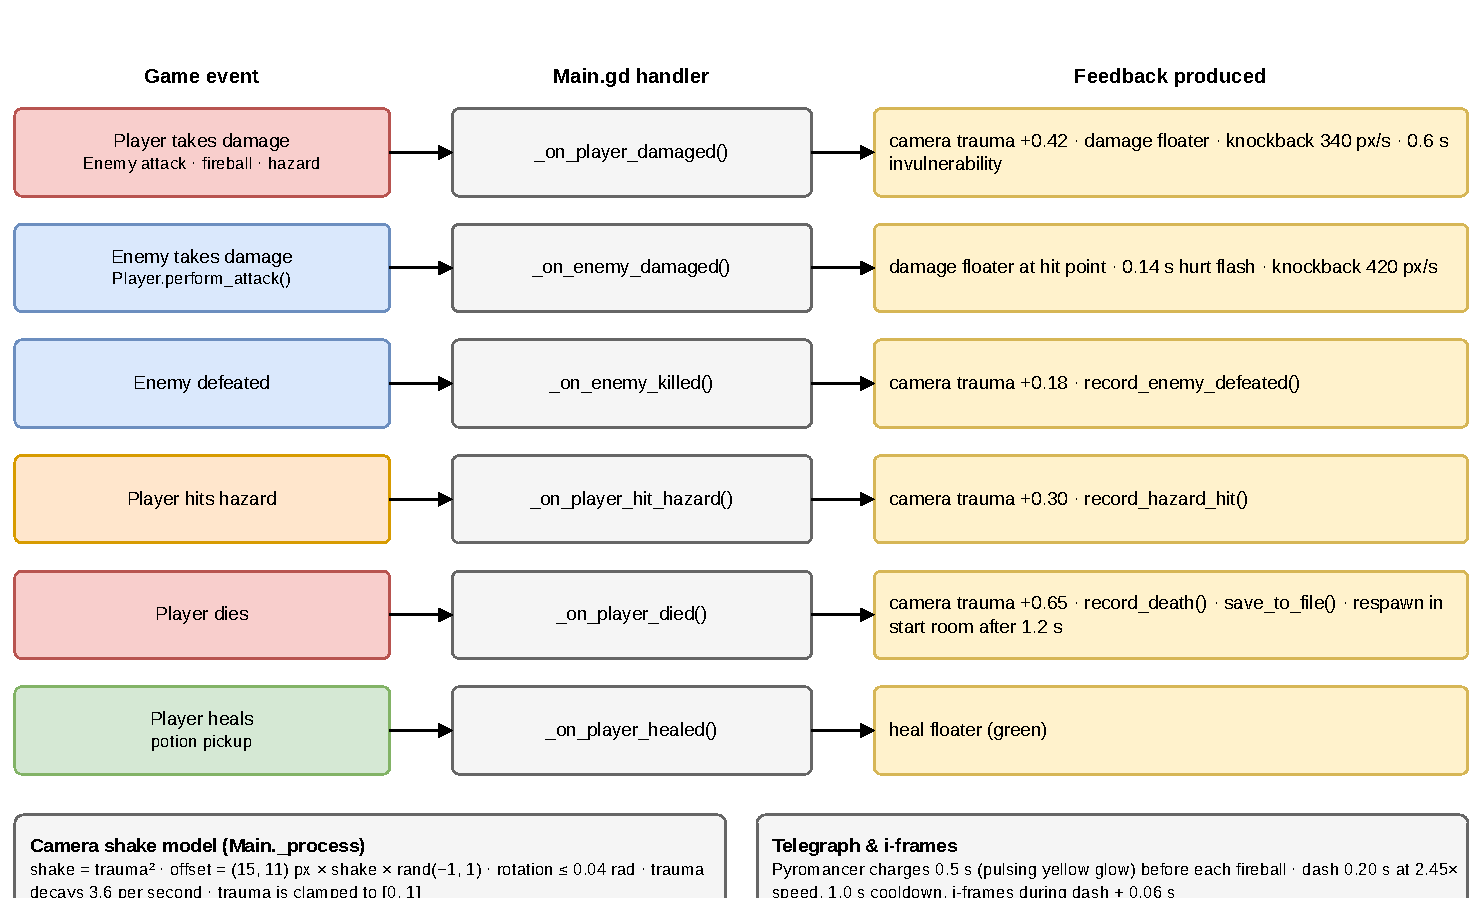
\includegraphics[width=0.95\textwidth]{ThesisFigs/fig_e_2_visual_asset_combat_feedback}
\caption{Combat Feedback Event Flow (event $\rightarrow$ handler $\rightarrow$ feedback)}
\label{fig:app_sprites}
\end{figure}
